%-*- coding: UTF-8 -*-
% author:wanghuai
% date:2020.12.28
% Jiangxi University of Science And Technology

% ========================
%|                        |
%|         导包			  |
%|                        |
% ========================

\documentclass[hyperref,UTF8]{ctexart}
%\usepackage{hyperref}
%\documentclass[unicode]{article}
%\usepackage[UTF8]{ctex}
% 导入PDF的包
\usepackage{float}
\usepackage{pdfpages} 
\usepackage{setspace}
\usepackage{fontspec}
\setmainfont{Times New Roman}
% 将章节序号改为中文
\usepackage{zhnumber} 
\renewcommand \thesection {\zhnum{section}}
\renewcommand \thesubsection {\arabic{section}.\arabic{subsection}}
% 设置页边距
\usepackage{geometry} 
\geometry{left=2.5cm,right=2.0cm,top=2.5cm,bottom=2.0cm}
% 设置页眉的包
\usepackage{fancyhdr} 
\pagestyle{fancy}	
\fancyhf{}
% 设置页码
\cfoot{\thepage}													

% 设置目录内容格式
\usepackage{titletoc}

\titlecontents{section}[0em]{\bfseries \zihao{4} \vspace{14.5pt}} {\contentslabel{2em}} {\hspace*{-2em}}{~\titlerule*[0.6pc]{$.$}~\contentspage}
\titlecontents{subsection}[2em]{\zihao{4} \vspace{14.5pt}} {\contentslabel{2em}} {\hspace*{-2em}}{~\titlerule*[0.6pc]{$.$}~\contentspage}
% 设置每节标题格式
\CTEXsetup[format={\raggedright \heiti \zihao{3} \bfseries}]{section} % 一级标题三号黑体加粗
\CTEXsetup[format={\raggedright \heiti  \zihao{4} \bfseries}, indent={0pc}]{subsection} % 二级标题四号黑体加粗

% 设置参考文献的包
\usepackage{gbt7714} % 使用GB/T-7714-2015格式


% ========================
%|                        |
%|         正文			  |
%|                        |
% ========================


\begin{document}
% 导入封面
%pdf修改为论文封面的PDF文件绝对路径名

\includepdf[pages=-]{/Users/wanghuai/Documents/研究生材料/开题报告/开题报告Latex模版/thesis_cover.pdf}


% 生成目录

% 取消目录的页眉
\fancyhead[L]{} % 设置学院
\fancyhead[R]{} % 设置姓名
\renewcommand{\headrulewidth}{0pt} 
% 目录两字中间空两格
\fontsize{14.5}{29}\selectfont
\renewcommand*\contentsname{\hfill 目\quad 录 \hfill} 
\tableofcontents
\setcounter{page}{1}						% 设置当前页页码编号从1开始计数
\pagenumbering{Roman}						% 设置页码字体为大写罗马字体

% 若要在目录后添加空白页,请将下面三行注释
%\newpage
%\thispagestyle{empty} % 当前页不显示页码
%\mbox
\newpage


% 正文字体(四号)、行间距(多倍行间距,1.25)
\fontsize{14.5}{18}\selectfont
% 段落间距为0
\setlength\parskip{0pt} % 取消段间距
% 设置页眉左右内容
\fancyhead[L]{江西理工大学} % 设置学院
\fancyhead[R]{信息工程学院\quad 张三} % 设置姓名
\renewcommand{\headrulewidth}{0.4pt} %设置页眉横线粗细
% 设置正文页码
\setcounter{page}{1}						% 设置当前页页码编号从1开始计数
\pagenumbering{arabic}						% 设置页码字体为小写阿拉伯字体


\section{ 选题背景与研究意义}
\subsection{研究背景}
在信息化时代的今天,高光谱遥感技术已经和人类工作生活息息相关。高光谱遥感突出特点和优势使其在众多领域发挥着越来越重要的作用,比如在军事目标侦查、阵地与装备伪装识别等。
\subsection{ 研究意义}
插入表格,如表(\ref{tab:label1})所示 \\
\begin{table}[H]
\centering
\caption{成绩单}
	\begin{tabular}{|c|r|r|r|p{4em}|}
	\hline
	姓名 & 语文 & 数学 & 外语 & 备注 \\
	\hline
	张三 & 87 & 100 & 93 & 优秀 \\
	张三 & 87 & 100 & 93 & 优秀 \\
	张三 & 87 & 100 & 93 & 优秀 \\
	\hline
\end{tabular}
\label{tab:label1}
\end{table}

\newpage
\section{国内外研究现状}
插入图片,如图\ref{fig:figure1} 所示 \\
\begin{figure}[H]
	\centering
	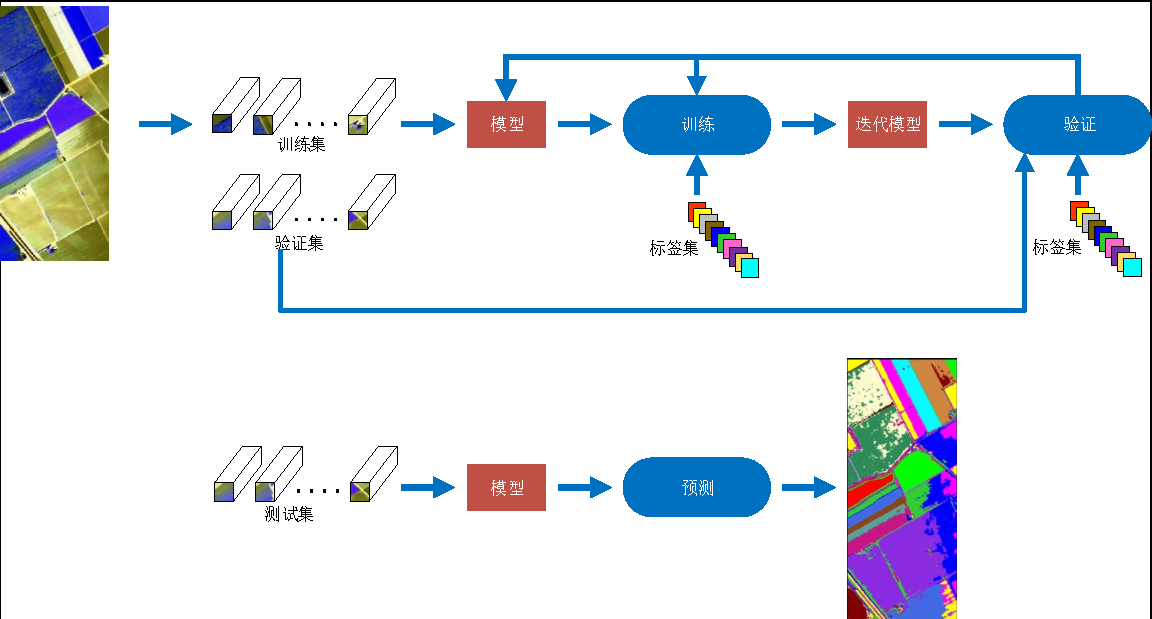
\includegraphics[scale=0.8]{CNN.pdf} % 为了是图片不失真,一般选择保存为 .pdf/.eps 格式插入
	\caption{深度学习应用于HSI分类一般流程}
	\label{fig:figure1}
\end{figure}


\section{课题研究内容与目标}
\subsection{研究内容}
插入公式(\ref{eq:eq1}) \\

\begin{equation}
	\centering
	a^2 = b^2 + c^2
	\label{eq:eq1}
\end{equation}


插入公式(\ref{eq:eq2}) \\
\begin{equation}
	\centering
	5^2 = 3^2 + 4^2
	\label{eq:eq2}
\end{equation}
	
\subsection{研究目标}

\section{技术路线}
高光谱遥感(Hyperspectral Remote Sensing,HSI)全称为高光谱分辨率遥感,起源于20世纪80年代。近年来,随着航空航天技术的飞速发展,遥感系统采集到的影像光谱分辨率得到极大提升,光谱分辨率可以达到纳米级,航天成像光谱仪能够在连续的几十个甚至几百个光谱波段获取地物辐射信息 \cite{张兵2017}。在取得地物空间图像同时,每个像元都能得到一条包含地物光谱特征的连续光谱曲线。

\section{拟解决关键问题和研究方案}
\subsection{拟解决关键问题}
\subsection{研究方案}

\section{特色与创新之处}

\section{论文进度安排}




\clearpage
\phantomsection										% 解决目录中超链接地址问题
\addcontentsline{toc}{section}{参考文献}				% 将参考文献添加到目录

\bibliographystyle{gbt7714-numerical}
\bibliography{math}
\end{document}